%03introduction.tex

\chapter{Motivation und Ausgangslage}
\section{Ein mobiles App f\"ur Feldforschung im Wald}
Aufbauend auf der existierenden "Waldmeister" App, welches von Studenten und Professoren als Nachschlagewerk f\"ur Waldstandortbestimmungen in der Praxis verwendet wird, existieren viele, teils digitalisierten Karten, welche den Stand der Forschung in sogenannten Vegetationskundlichen Karten beschreiben. Waldstandortbestimmung ist ein sich st\"andig im Wechsel befindendes Thema und auch in der Schweiz k\"onnen sich Standorte oder deren Befund \"uber Jahre \"andern. Vegetationskundliche Karten, welche von Experten im Auftrag des Kantons angefertigt werden, befinden sich in statischen oder ungewarteten Zust\"anden in Archiven des Kantons, oder werden in grossen Intervallen (5-10 Jahre) revidiert. Teilweise sind diese Daten daher gar nich, oder nur oder in sehr veralteten Zustand zug\"anglich.
Dies liegt haupts\"achlich am grossen Kostenaufwand welche eine Analyse im Feld durch Experten mit sich bringt. Der Datenfluss ist gepr\"agt von analogen Vorg\"angen, vorallem da viele technische Ger\"ate nicht f\"ur den Einsatz im Feld geeignet sind und kantonale Organisationen als Mittelsm\"anner etabliert sind, welche die Daten von Experten archivieren und ggf. in digitaler Form ver\"offentlichen. "Waldmeister - Outdoors" zielt darauf hin den Arbeitszyklus der Analyse und Publikation von Waldstandorten zu vereinfachen und zu beschleunigen. Dies soll erreicht werden durch neue technische M\"oglichkeiten und Medien wie dem Smartphone, GPS und Mobiles Internet.\"u
Das Instrument "Waldmeister - Outdoors" soll dazu verwendet werden die Erfassung von Geoinformationsdaten bez\"uglich der Waldstandortbestimmung zu standardisieren und deren \"ubermittlung an die zust\"andige Beh\"orde, Forschern und anderen Experten zu beschleunigen. Anstelle eines Jahrelangen Projekts, einen Bestimmten Standort in Waldstandorte zu kategorisieren, soll ein System entwickelt werden, welches eine inkrementelle digitale Erfassung und Publikation erm\"oglicht, den Arbeitsaufwand der Experten erleichtert und den Informationsaustausch, - und Abgleich beschleunigt.

\section{Use Cases}
\subsection{Zugriff auf Vegetationskundliche Karten}
W\"ahrend der Feldforschung kann es sehr hilfreich sein auf bereits kategorisierte Waldfl\"achen Zugriff zu haben um sich am Standort zu orientieren. Dieses Material ist oft in einem Kantonalen Portal z.B. https://maps.zh.ch erh\"altlich, sind jedoch nur selten kompatibel mit mobilen Ger\"aten, interagieren nicht mit dem GPS des Smartphones oder die Webseiten sind schwer zu navigieren. "Waldmeister-Outdoors" soll einem gezielten Zweck dienen und nicht mit Kartenmaterial \"uberladen werden um den Zugriff auf die Vegetationskundliche Karten zu vereinfachen und die Navigation zu beschleunigen. $\newline

\subsection{Bearbeitung der Vegetationskundlichen Karten}
Kantonale Vegetationskundliche Karten sind statisch (d.h. Read-Only) und k\"onnen von Usern nicht bearbeitet oder erweitert werden. Dies f\"uhrt dazu dass Kartenmaterial in veraltetem Zustand vorliegt und Fehler oder Ver\"anderungen nur mit grossem Aufwand upgedatet werden k\"onnen. Nicht nur f\"uhrt dies zu Problemen bei der Kommunikation mit anderen Experten, Forschern und Studenten, es behindert auch den Arbeitsfluss der Person, welche sich im Feld befindet, da andere Mittel zur tempor\"aren Festhaltung der Ergebnisse verwendet werden m\"ussen, um an einem sp\"ateren Zeitpunkt wieder darauf zugreifen zu k\"onnen (z.B. eine halbj\"ahrliche Untersuchung eines Standorts, ohne die Zwischenergebnisse zu publizieren). Dies geschieht oft analog, auf Papier im Feld und kann zu einem sp\"ateren Zeitpunkt zum pers\"onlichen Gebrauch digitalisiert werden, was zu einem erh\"ohten Arbeitsaufwand f\"uhrt. Durch die Verwendung von "Waldmeister - Outdoors" kann das gleiche Werkzeug ben\"utzt werden um eine Fl\"ache w\"ahrend der Untersuchung sowohl im Feld als auch im B\"uro zu beschreiben, sowie die finalen Befunde am Ende der Untersuchung zu publizieren und zu Teilen.

\subsection{Unterst\"utzung w\"ahrend der Untersuchung}
Feldforschung hat oft mit der Orientierung und der Man\"ovrierung des Standorts an sich zu tun und auch hier kann "Waldmeister - Outdoors" den Arbeitsaufwand simplifizieren und reduzieren. Durch die direkte digitale Erfassung von beliebigen Notizen bez\"uglich dem Standort m\"ussen diese nicht mehr analog erfasst werden und k\"onnen direkt der Position in der realen Welt zugeordnet werden. Ist Beispielsweise ein Gebiet schwer Befahrbar oder zug\"anglich kann dies direkt auf der digitalen Karte erfasst und f\"ur pers\"onliche Zwecke gespeichert werden, k\"onnen aber ebenfalls publiziert werden falls sie f\"ur Andere von Interesse sind. Es kann sich hierbei auch um Pfade oder einzelne Standorte von Indikatoren handeln, bzw. eine genaue Lage der Observationsfl\"ache welche untersucht werden soll.

\subsection{Automatische Bestimmung einer Waldfl\"ache}
Durch den Zugriff auf eine Datenbank, in welcher jede Waldstandort einem Typ zugeordnet ist, kann mithilfe des Mobilen Ger\"ats der Typ des Waldstandorts in welcher sich ein User gerade befindet automatisch bestimmt werden. Dies kann mithilfe des GPS Sensors des Mobilen Ger\"ats und einer Datenbankabfrage zu jedem Zeitpunkt geschehen.

\section{Mobile Limits}
In vielen F\"allen ist eine Standortbestimmung durch GPS im Wald sehr ungenau und die Internetverbindung kann instabil sein. Im Idealfall \"ubertr\"agt das Werkzeug so wenig Daten wie m\"oglich, speichert diese auf dem Ger\"at und wartet auf eine stabile Verbindung um Daten auf den Server zu \"ubertragen. $\newline$
Kartenmaterial sollte wenn m\"oglich permanent auf das Mobile Ger\"at geladen werden k\"onnen, damit Datenvolumen bei der Verwendung im Feld nicht strapaziert werden.

\chapter{Technologies}
\section{Progressive Webapp}
Um das Werkzeug "Waldmeister - Outdoors" nicht auf eine Platform von Mobilen Ger\"aten zu beschr\"anken, setzt es auf die Prinzipien der Progressive Webapps (PWA). Es beschreibt eine Webseite welche viele Merkmale besitzt, welche bisher den nativen Apps vorbehalten waren. Eine PWA ist gewissermassen eine responsive Website, welche auch offline verwendet werden kann und schliesst dadurch eine zus\"atzliche Entwicklung einer nativen App, parallel zur Webseite \"uberfl\"ussig. Eine PWA erreicht diese offline F\"ahigkeiten durch den Einsatz von Service Workern; ein JavaScript welches von Web-Browsern im Hintergrund ausgef\"uhrt wird. Einmal online aufgerufen, k\"onnen die Inhalte beim n\"achsten Besuch der Seite auch dann angezeigt werden, wenn eine schlechte oder sogar gar keine Internetverbindung besteht (Offline-Betrieb). Auch die von nativen Apps bekannten Push-Benachrichtigungen sind mit Service Workern m\"oglich. \cite{ServiceWorkers} $\newline$
Grundlegende Charakteristiken der PWA sind Offline Funktionalit\"at, Push Notifications, Add-To-Homescreen, jedoch ist keine Installation notwendig (beispielsweise \"uber den Apple Appstore oder Google Playstore). Verbreitete Mobile Browser wie Firefox und Google Chrome haben bereits eine vollst\"andige Unterst\"utzung von PWAs, Safari sollte dies bis Ende Februar 2018 ebenfalls implementiert haben und kann daher auch auf iOS verwendet werden.

\section{ESRI / ArcGIS online}
Technologien von ESRI und insbesondere ArcGIS online wurden recherchiert um einen funktionierenden Prototypen mit offline-caching zu erstellen. Hintergrundkarten (in Form einen Tile-Layers) k\"onnen auf dem Ger\"at zwischengespeichert werden, und die Erstellung und Synchronisation von editierbaren Vektorlayern funktioniert auch beim offline Betrieb. Vektorlayer k\"onnen Punkte, Pfade oder Fl\"achen beschreiben und k\"onnen offline erstellt werden und werden bei verf\"ugbaren Internetverbindung mit einem Server synchronisiert.

\section{Vue.JS}
Vue.JS ist ein JavaScript framework welches sich zum Erstellen von Single-Page Webapplikationen eignet. Es wurde im Jahr 2013 erstmals ver\"offentlicht und wurde am 19. Dezember 2017 auf die aktuellsten Version 2.5.13 gepatcht. Vue.JS folgt einer Variation des Model-View-Controller Entwurfmusters genannt dem Model - View - ViewModel Muster. Wie auch das MVC folgt MVVM dient es der Trennung von Darstellung und der Logik der Benutzerschnittstelle. Dies erlaubt dem nutzenden Entwickler, die Struktur der Anwendung nach eigenen Anspr\"uchen zu richten.Entwickler beschreiben es daher als "less opinionated" im Vergleich zu anderen popul\"aren JavaScript Webframeworks wie Anglar.JS und React. Vue.JS kann von Entwicklern eingesetzt werden welche HTML und JavaScript beherrschen und erfordert keine weiteren Webtechnologien. Vue.JS setzt eine Webseite aus Instanzen und Komponenten, bzw Single File Components zusammen.

\subsection{Vue-Router}
Der Vue-Router ist das Herzst\"uck einer Single-Page-Applikation (SPA). Der Vue-Router bestimmt unter welchen Routen welche Komponenten gerendert werden sollen. In der HTML Definition der Haupkomponente kann <router-view> als Platzhalter verwendet werden um die Komponenten anzuzeigen, welche abh\"angig von der momentanen Route an dieser Stelle angezeigt werden sollen. Ein Wechsel zwischen diesen Routen bewirkt kein Page-Reload, da dies von Vue.JS lediglich innerhalb derselben Page \"anderungen bewirkt und keine tats\"achlichen URL Aufrufe ausf\"uhrt.

\subsection{VueX}
VueX ist eine offizielle Erweiterung von Vue.JS und fungiert als Statusmanager. VueX arbeitet mit einem Store welcher die Zust\"ande aller Komponenten in einer Vue Applikation \"uber Regeln definiert. VueX besteht aus Actions, Mutations und States, und Aktionen k\"onnen in dieser Reihenfolge eine Auswirkung auf die Vue Komponenten haben. $\newline$
VueX hat Vorteile bei mittel bis grossen Projekten welche auf dem Single-Page-Application Prinzip basieren. VueX bietet auch die M\"oglichkeit einen zentralen Store in kleinere Module aufzuteilen, jedes mit ihrer eigenen State, Mutations, Actions Werten.
\begin{figure}[h]
    \centering
    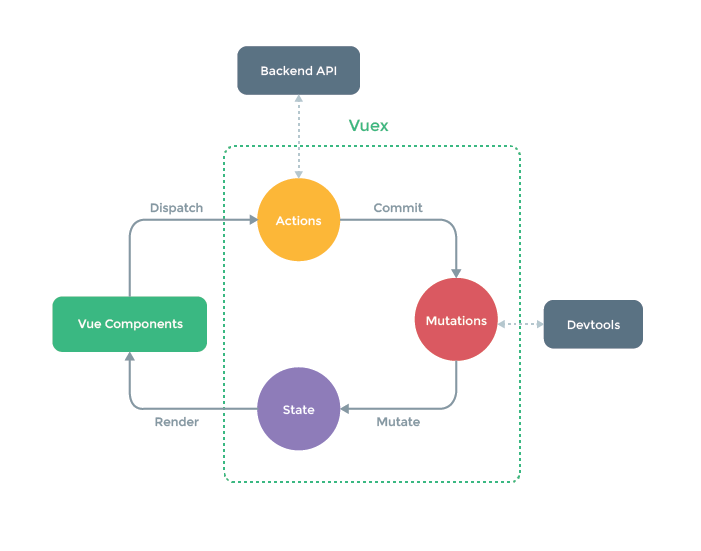
\includegraphics[width=1.25\textwidth]{vuex}
    \caption{Vuex Action-Mutations-State Diagram}
    \label{fig:mesh1}
\end{figure}


\subsection{Vuetify}
Vuetify ist eine Vue.JS UI Framework welches das Frontend aus vielen, Material-Design basierten UI Bausteinen zusammenbaut.

\section{Axios}
Axios ist eine JavaScript library welche Promise-Based HTTP Requests, welche "Waldmeister-Outdoors" dazu verwendet mit dem Server zu kommunizieren. Axios erm\"oglicht es asynchrone HTTP requests zu REST Endpunkten abzusetzen oder CRUD Operationen auszuf\"uhren. Axios kann in puren JavaScript Projekten verwendet werden oder auch in Projekten welche auf Vue.JS basieren. Ein Promise-Objekt repr\"asentiert die in der Zukunft geschehende Komplettierung einer asynchronen Operation (oder deren Abbruch durch einen Fehler).

\section{Django}
Als Server zur Verwaltung der User und der Daten welche die User generieren und ben\"otigen kommt Django zum Einsatz. Es ist ein Open-Source Webframework welches das Python Gegenst\"uck zu Ruby-On-Rails darstellt. Im Kern folgt es dem Model-View-Controller Prinzip, obwohl es eigene Namensgebung f\"ur diese Verwendet. Django verwendet eine PostgreSQL Datenbank um Daten persistent zu machen. Django wird ebenfalls dazu verwendet um User einen Account zu geben, damit nur sie Zugriff auf Ihre privaten Fl\"achen haben, bevor sie vom User ver\"offentlich werden.
\subsection{Django Rest Framework}
Da eine SPA haupts\"achlich \"uber API Schnittstellen mit dem Server kommuniziert, wird auf dem Server das Django Rest-Framework (DRF) eingesetzt. Es bietet ein sehr flexibles System zur Erstellung von RESTful Web-APIs. Das DRF bietet die M\"oglichkeiten GET, POST, PUT und DELETE auf eine Resource auszuf\"uhren. "Waldmeister-Outdoors" verwendet die REST Api beispielsweise um usergenerierte Fl\"achen, Pfade oder Punkte in die Datenbank zu speichern oder diese zur Darstellung in der Map aus der Datenbank zu laden. Ebenfalls werden Benutzer welche sich Registrieren mit Username, Password und ggf. Emailadresse in der Datenbank eingetragen. $\newline$

\section{PostgreSQL}
Postgres ist das Datenbank Management System welches mit Django zusammen die Daten persistent macht, welche die User per API in der PWA generieren. Hierzu wird das Django Packet Psycopg2 verwendet. Django kann durch Models ein Datenbankschema beschreiben, welches von PostgreSQL generiert und in einer lokalen PostgreSQL Instanz gespeichert wird.
\subsection{PostGIS}
Um Geoinformationsdaten wie z.B. Polygone und Pfade korrekt zu speichern wird auf der Datenbank das Plugin PostGIS installiert. Dadurch kann Django die ben\"otigten Datenbankmodelle erstellen und per REST Schnittstelle speichern. 


\section{Leaflet}
Leaflet ist eine JavaScript Library welche es erm\"oglicht Map auf dem Client darzustellen. Es fokussiert sich auf Simplizit\"at, Performanz und ist sehr schlank, was einer PWA sehr entgegen kommt. Die Library ist nur 38 KB gross und erm\"oglicht es viele Features welche bei der Darstellung einer Map ben\"otigt wird zu verwenden. 

\subsection{TileLayer}
Der TileLayer fungiert als Hintergrundkarte welche dynamisch geladen wird. Je nach ben\"otigtem Kartenausschnitt werden die Tiles als .pngs geladen und auf der Karte dargestellt. Dies f\"uhrt dazu dass je nach Gr\"osse und Zoomstufe des Kartenausschnitts nur minimalen Datenaufwand bet\"atigt wird. Als Hintergrundkarte werden die "terrain" Tiles von "stamen-tiles" verwendet.

\subsection{Leaflet editable}
Damit die User neue Polygone, Punkte und Pfade erfassen k\"onnen ben\"otigt Leaflet das Plugin "Leaflet editable", welches es erm\"oglicht neue Objekte direkt auf der Map zu zeichnen, oder bestehende Objekte zu editieren. Sobald ein Objekt abgeschlossen ist, wird es per REST Schnittstelle an die Datenbank \"ubertragen. Der User hat die M\"oglichkeit de Objekt einen Namen als Label zuzuweisen, und es zwischen privat oder public zu wechseln. Jeder User hat nur Zugriff auf seine eigenen privaten Fl\"achen, bzw. Pfade und Punkte, ausser er w\"ahlt es diese zu Ver\"offentlichen, bzw "public" zu machen, damit sie alle User auf der Map sehen.

\chapter{Implementation}

\section{Mockup}
Die Mockups wurden vor der Implementation erstellt um das Screendesign und Layout klarer zu definieren bevor es um die technische Implementation von "Waldmeister - Outdoors" ging. In den Abbildungen 1 bis 9 kann man den Arbeitsschritt Einloggen und Erstellen einer neuen Fl\"ache und eines Points of Interests (POI) sehen. Zus\"atzlich sieht der User seine eigene Location auf der Map eingetragen und hat \"uber das Menu "My Places" Zugriff auf eine Liste seiner erstellten Fl\"achen. Ein Kontextmenu gibt bei der Anzeige eines bestimmten Objekts zus\"atzliche Informationen \"uber dieses.

\begin{figure}[h]
\centering
    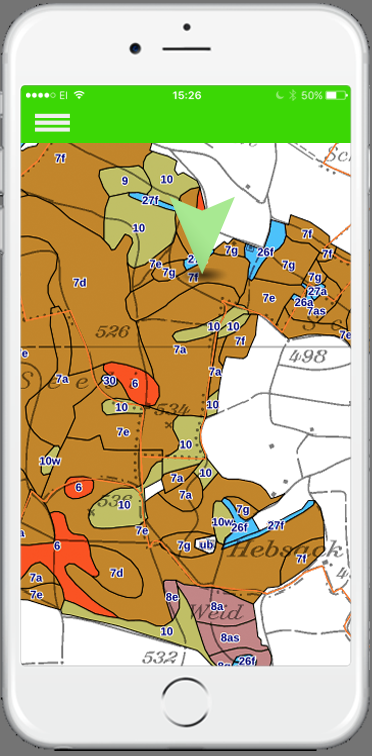
\includegraphics[width=0.7\textwidth]{mockup1-1}
    \caption{Mockup Screen 1}
    \label{fig:mesh1}
\end{figure}

\begin{figure}[h]
\centering
    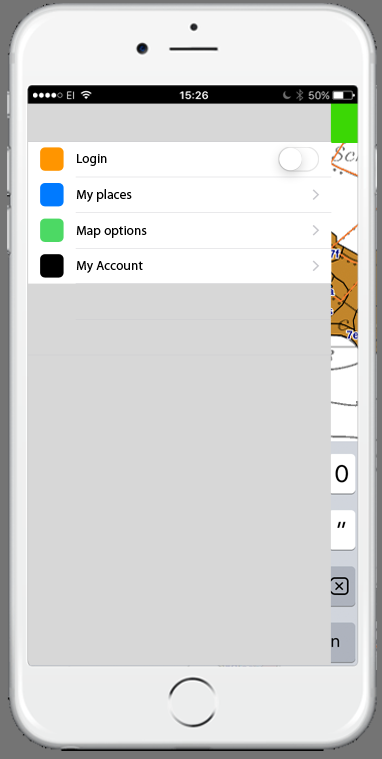
\includegraphics[width=0.7\textwidth]{mockup1-2}
    \caption{Mockup Screen 2}
    \label{fig:mesh2}
\end{figure}

\begin{figure}[h]
\centering
    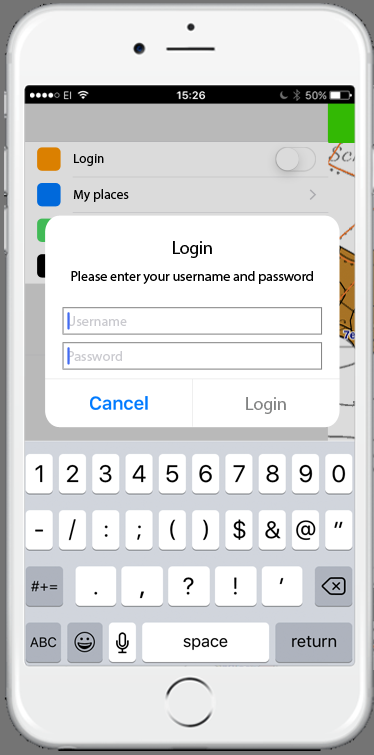
\includegraphics[width=0.7\textwidth]{mockup1-3}
    \caption{Mockup Screen 3}
    \label{fig:mesh3}
\end{figure}

\begin{figure}[h]
\centering
    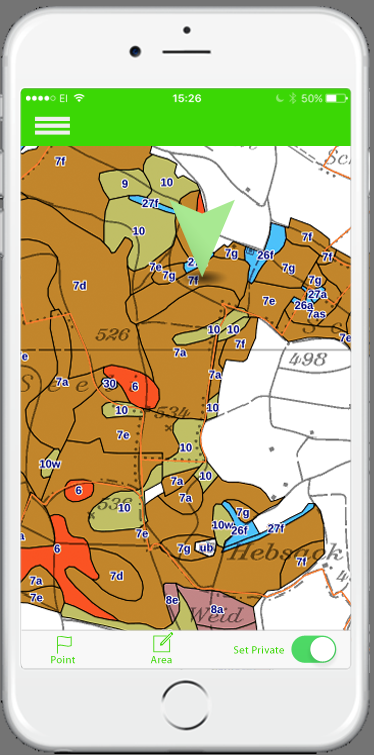
\includegraphics[width=0.7\textwidth]{mockup1-4}
    \caption{Mockup Screen 4}
    \label{fig:mesh4}
\end{figure}

\begin{figure}[h]
\centering
    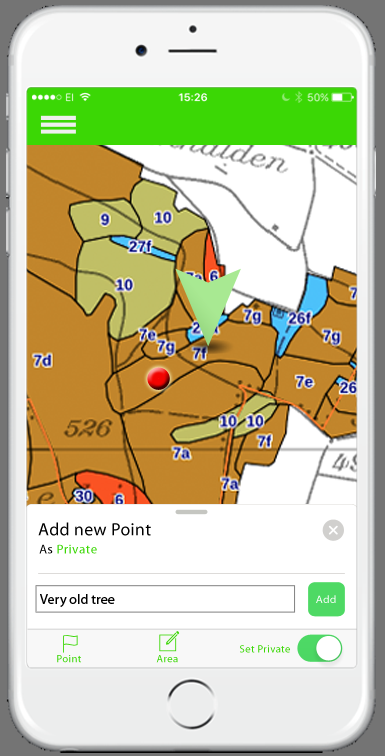
\includegraphics[width=0.7\textwidth]{mockup1-5}
    \caption{Mockup Screen 5}
    \label{fig:mesh5}
\end{figure}

\begin{figure}[h]
\centering
    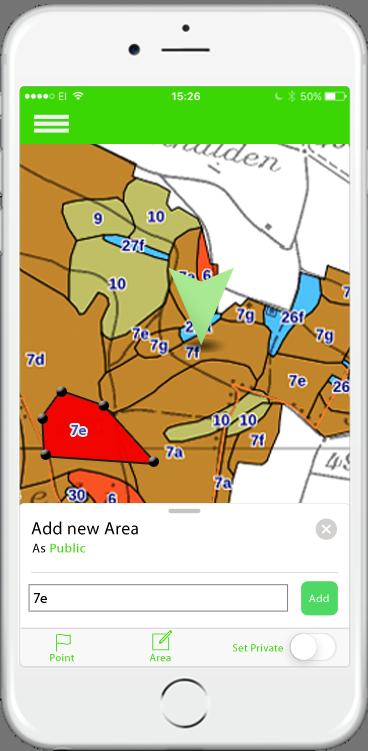
\includegraphics[width=0.7\textwidth]{mockup1-6}
    \caption{Mockup Screen 6}
    \label{fig:mesh6}
\end{figure}

\begin{figure}[h]
\centering
    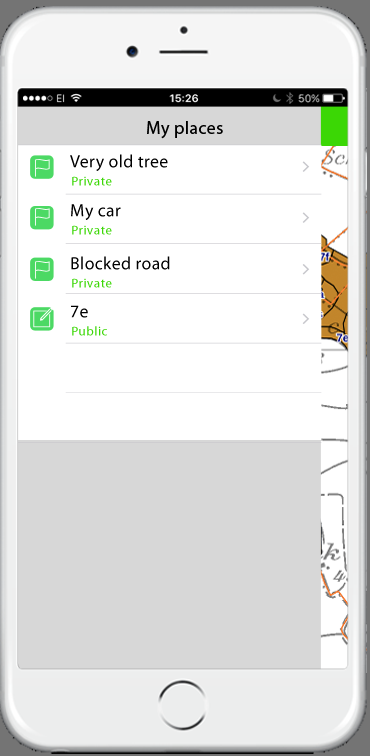
\includegraphics[width=0.7\textwidth]{mockup1-7}
    \caption{Mockup Screen 7}
    \label{fig:mesh7}
\end{figure}

\begin{figure}[h]
\centering
    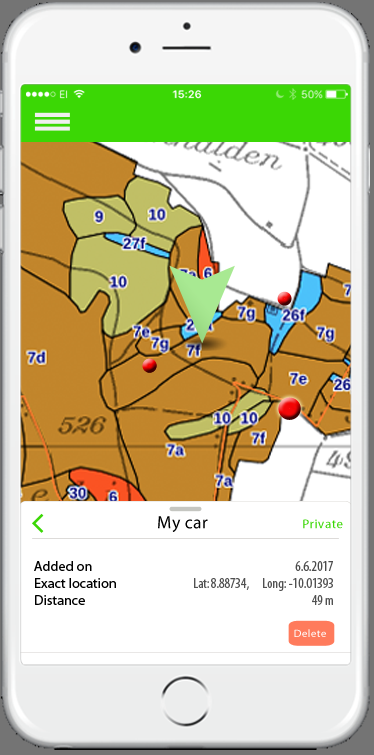
\includegraphics[width=0.7\textwidth]{mockup1-8}
    \caption{Mockup Screen 8}
    \label{fig:mesh8}
\end{figure}

\begin{figure}[h]
\centering
    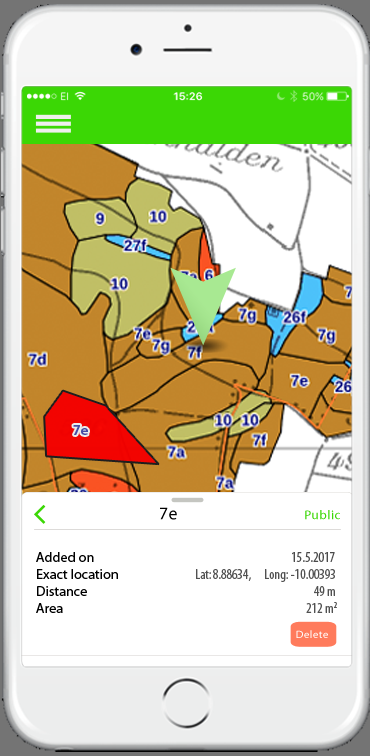
\includegraphics[width=0.7\textwidth]{mockup1-9}
    \caption{Mockup Screen 9}
    \label{fig:mesh9}
\end{figure}



\section{UMLs}
UML Diagramme geben Auskunft \"uber die Architektur und innere Abl\"aufe des Systems

\subsection{Use Case - Diagramm}
Das Diagram \ref{fig:uc1} zeigt auf welche M\"oglichkeiten ein User hat mit dem Werkzeug zu interagieren. Ein User welcher sich nicht registriert kann weder Fl\"achen generieren oder editieren und kann keine privaten Fl\"achen sehen. Er kann jedoch die Vegetationskundliche Karte und \"offentliche Fl\"achen aller anderen User sehen. Erst wenn er sich einloggt kann er seine eigenen privaten und \"offentlichen Fl\"achen editieren oder erstellen.
\begin{figure}[h]
\centering
    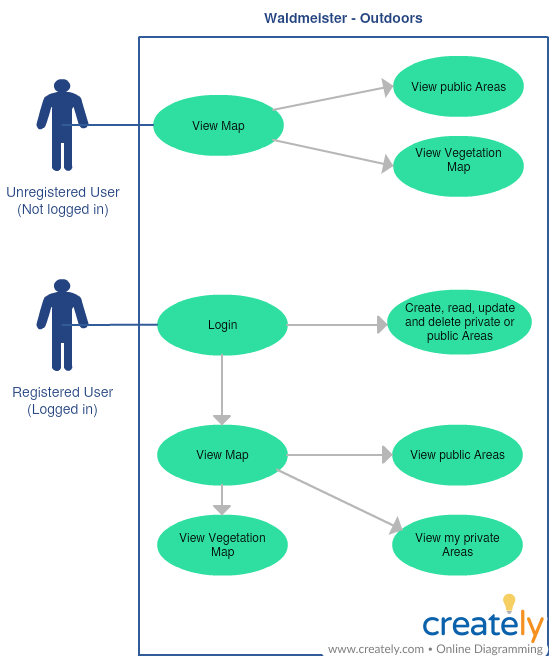
\includegraphics[width=0.9\textwidth]{WaldmeisterMap_USECASE}
    \caption{Use Case Diagram}
    \label{fig:uc1}
\end{figure}

\subsection{Klassendiagram, Datenbankdiagramm}
Das Diagramm \ref{fig:cd1}  schildert die Relation und Ausbau der wichtigsten zwei Klassen des Systems.

\begin{figure}[h]
\centering
    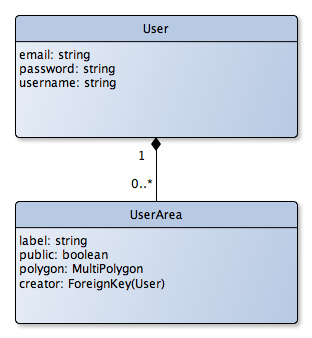
\includegraphics[width=0.5\textwidth]{ClassDiagram2}
    \caption{Klassendiagramm}
    \label{fig:cd1}
\end{figure}

\subsection{Sequenzdiagramm}

Die folgenden Sequenzdiagramme geben detaillierten Einblick in den Ablauf des Registrierung, - und Loginvorgangs sowie das Laden der Public und Private Areas und deren Darstellung im Client. $\newline$

\begin{figure}[h]
\centering
    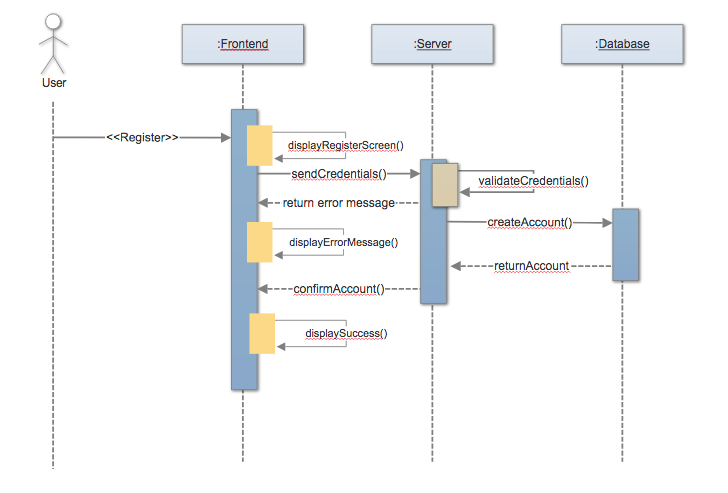
\includegraphics[width=0.9\textwidth]{Sequenz_DiagrammRegister}
    \caption{Sequenzdiagramm, Register}
    \label{fig:sd1}
\end{figure}

\begin{figure}[h]
\centering
    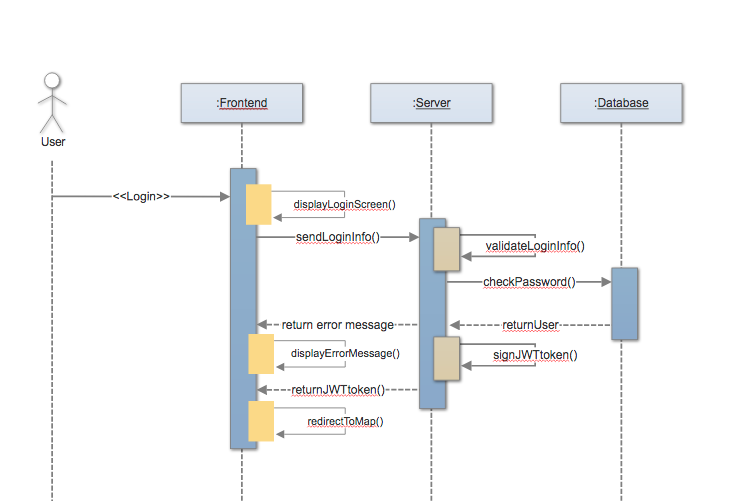
\includegraphics[width=0.9\textwidth]{Sequenz_DiagrammLogin}
    \caption{Sequenzdiagramm, Login}
    \label{fig:sd2}
\end{figure}

\begin{figure}[h]
\centering
    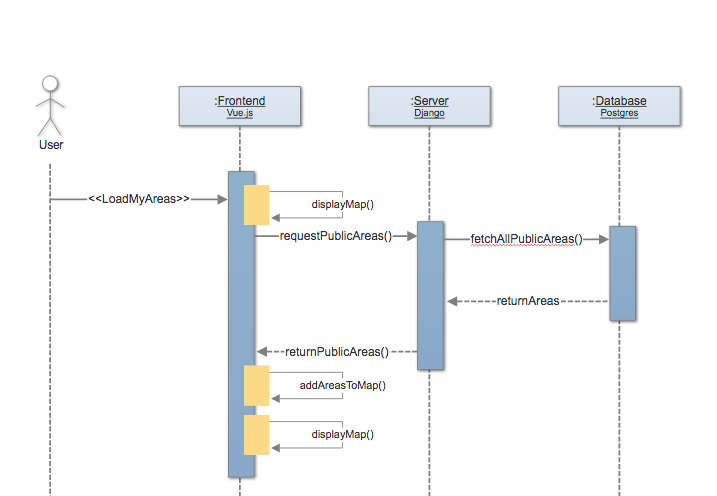
\includegraphics[width=0.9\textwidth]{Sequenz_DiagrammPublicAreas}
    \caption{Sequenzdiagramm, Public Areas}
    \label{fig:sd3}
\end{figure}

\begin{figure}[h]
\centering
    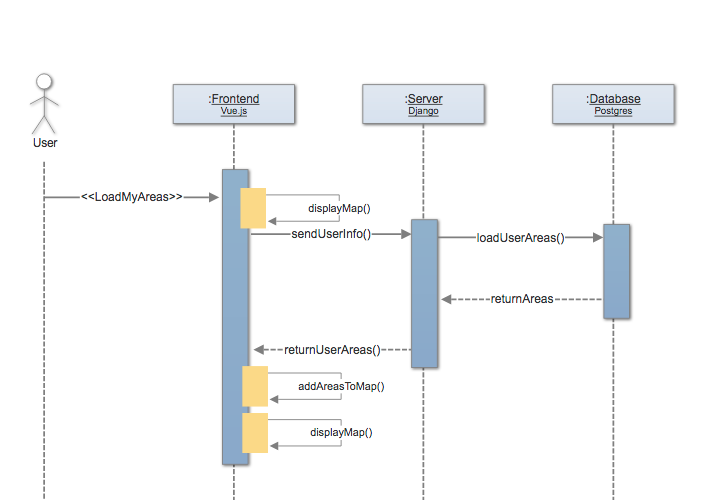
\includegraphics[width=0.9\textwidth]{Sequenz_DiagrammMyAreas}
    \caption{Sequenzdiagramm, My Areas}
    \label{fig:sd4}
\end{figure}


\chapter{Results}
Das Projekt wurde mit genannten Technologien umgesetzt und wird auf Github gehostet: $\newline$

https://github.com/dschmide/Waldmeister

$\newline$


\section{Discussion /  Screenshots}

\begin{figure}[h]
\centering
    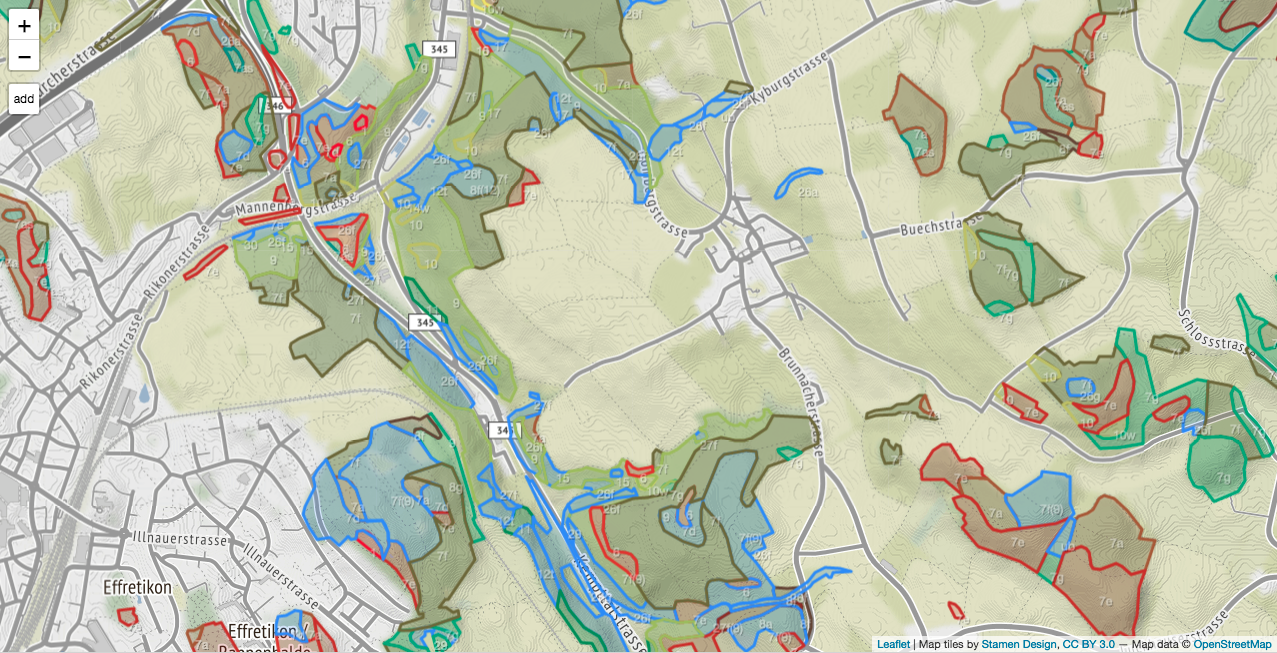
\includegraphics[width=1.1\textwidth]{ScreenShot}
    \caption{Screenshot Desktop, Vegetationskundliche Karte}
    \label{fig:ss1}
\end{figure}

\begin{figure}[h]
\centering
    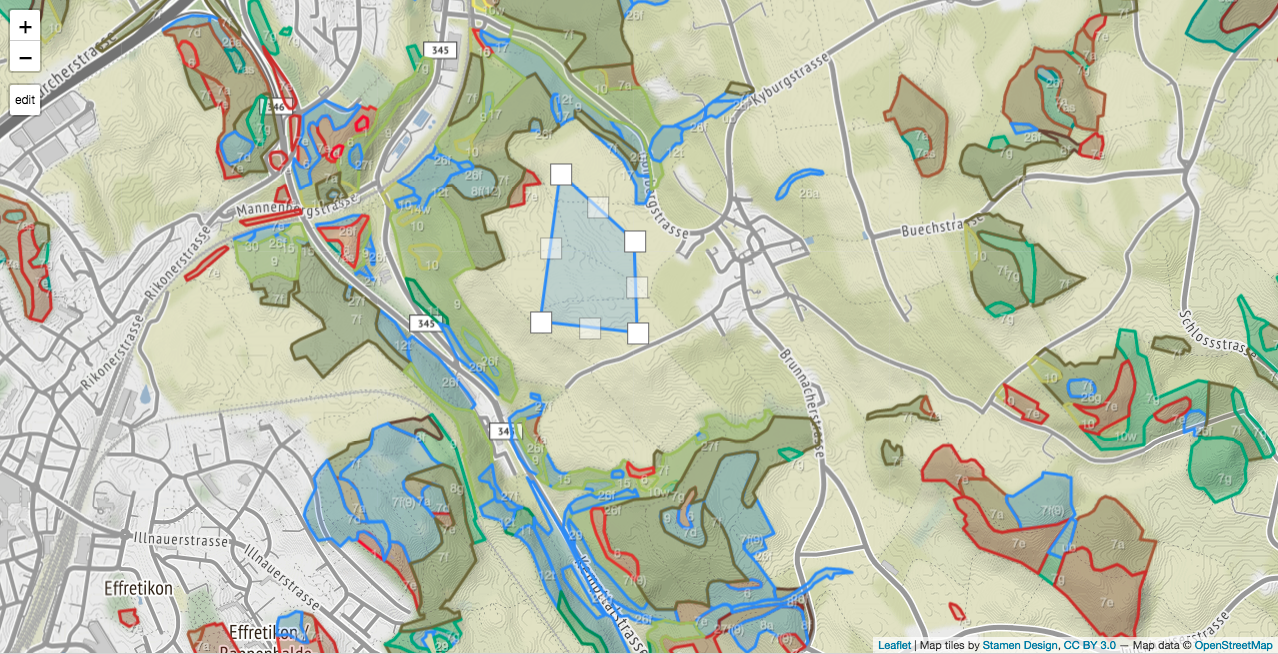
\includegraphics[width=1.1\textwidth]{ScreenShot2}
    \caption{Screenshot Desktop, EditArea}
    \label{fig:ss2}
\end{figure}


\chapter{Links}
https://github.com/dschmide/Waldmeister $\newline$
https://maps.zh.ch?topic=WaldVKZH&scale=18634&x=2706590.13&y=1251180.39&srid=2056

\chapter{API Documentation}





